\documentclass[12pt]{aghdpl}
% \documentclass[en,11pt]{aghdpl}  % praca w języku angielskim

% Lista wszystkich języków stanowiących języki pozycji bibliograficznych użytych w pracy.
% (Zgodnie z zasadami tworzenia bibliografii każda pozycja powinna zostać utworzona zgodnie z zasadami języka, w którym dana publikacja została napisana.)
\usepackage[english,polish]{babel}

% Użyj polskiego łamania wyrazów (zamiast domyślnego angielskiego).
\usepackage{polski}

\usepackage[utf8]{inputenc}

% dodatkowe pakiety

\usepackage{mathtools}
\usepackage{amsfonts}
\usepackage{amsmath}
\usepackage{amsthm}
\usepackage{array}
\usepackage{tabularx}

\newenvironment{conditions}
{\par\vspace{\abovedisplayskip}\noindent
\tabularx{\textwidth}{>{$}l<{$} @{${}={}$} >{\raggedright\arraybackslash}X}}
{\endtabularx\par\vspace{\belowdisplayskip}}


% --- < bibliografia > ---

\usepackage[
backend=biber,
style=numeric,
sorting=none,
%
% Zastosuj styl wpisu bibliograficznego właściwy językowi publikacji. 
language=autobib,
autolang=other,
% Zapisuj datę dostępu do strony WWW w formacie RRRR-MM-DD.
urldate=iso8601,
% Nie dodawaj numerów stron, na których występuje cytowanie.
backref=false,
% Podawaj ISBN.
isbn=true,
% Nie podawaj URL-i, o ile nie jest to konieczne.
url=false,
%
% Ustawienia związane z polskimi normami dla bibliografii.
maxbibnames=3,
]{biblatex}

\usepackage{csquotes}
% Ponieważ `csquotes` nie posiada polskiego stylu, można skorzystać z mocno zbliżonego stylu chorwackiego.
\DeclareQuoteAlias{croatian}{polish}

\addbibresource{bibliografia.bib}

% Nie wyświetlaj wybranych pól.
%\AtEveryBibitem{\clearfield{note}}


% ------------------------
% --- < listingi > ---

% Użyj czcionki kroju Courier.
\usepackage{courier}

\usepackage{listings}
\lstloadlanguages{TeX}

\lstset{
	literate={ą}{{\k{a}}}1
           {ć}{{\'c}}1
           {ę}{{\k{e}}}1
           {ó}{{\'o}}1
           {ń}{{\'n}}1
           {ł}{{\l{}}}1
           {ś}{{\'s}}1
           {ź}{{\'z}}1
           {ż}{{\.z}}1
           {Ą}{{\k{A}}}1
           {Ć}{{\'C}}1
           {Ę}{{\k{E}}}1
           {Ó}{{\'O}}1
           {Ń}{{\'N}}1
           {Ł}{{\L{}}}1
           {Ś}{{\'S}}1
           {Ź}{{\'Z}}1
           {Ż}{{\.Z}}1,
	basicstyle=\footnotesize\ttfamily,
}

% ------------------------

\AtBeginDocument{
	\renewcommand{\tablename}{Tabela}
	\renewcommand{\figurename}{Rys.}
}

% ------------------------
% --- < tabele > ---

\usepackage{array}
\usepackage{tabularx}
\usepackage{multirow}
\usepackage{booktabs}
\usepackage{makecell}
\usepackage[flushleft]{threeparttable}

% defines the X column to use m (\parbox[c]) instead of p (`parbox[t]`)
\newcolumntype{C}[1]{>{\hsize=#1\hsize\centering\arraybackslash}X}


\newenvironment{abstractpage}
{\cleardoublepage\vspace*{\fill}\thispagestyle{empty} }
{\vfill\cleardoublepage}
\renewenvironment{abstract}[1]
{\bigskip\selectlanguage{#1}%
	\begin{center}\bfseries\abstractname\end{center}}
{\par\bigskip}


%---------------------------------------------------------------------------

\author{Tomasz Kańka}
\shortauthor{T. Kańka}

%\titlePL{Przygotowanie bardzo długiej i pasjonującej pracy dyplomowej w~systemie~\LaTeX}
%\titleEN{Preparation of a very long and fascinating bachelor or master thesis in \LaTeX}

\titlePL{Sprzętowo-programowy system wizyjny do detekcji obiektów zwykorzystaniem termowizji}
\titleEN{Hardware-software vision system for object detection with the use of thermovision.}


\shorttitlePL{Sprzętowo-programowy system wizyjny do detekcji obiektów z wykorzystaniem termowizji} % skrócona wersja tytułu jeśli jest bardzo długi
\shorttitleEN{Hardware-software vision system for object detection with the use of thermovision.}

\thesistype{Praca dyplomowa magisterska}
%\thesistype{Master of Science Thesis}

\supervisor{dr inż. Tomasz Kryjak}
%\supervisor{Marcin Szpyrka PhD, DSc}

\degreeprogramme{Automatyka i Robotyka}
%\degreeprogramme{Computer Science}

\date{2018}

\department{Katedra Automatyki i Robotyki}
%\department{Department of Applied Computer Science}

\faculty{Wydział Elektrotechniki, Automatyki,\protect\\[-1mm] Informatyki i Inżynierii Biomedycznej}
%\faculty{Faculty of Electrical Engineering, Automatics, Computer Science and Biomedical Engineering}

%TODO uzupełnić lub usunąć
\acknowledgements{Serdecznie dziękuję \dots tu ciąg dalszych podziękowań np. dla promotora, żony, sąsiada itp.}


\setlength{\cftsecnumwidth}{10mm}

%---------------------------------------------------------------------------
\setcounter{secnumdepth}{4}

\begin{document}

\titlepages

\begin{abstractpage}
	\begin{abstract}{polish}

		
		\textbf{Słowa kluczowe:} 
		
	\end{abstract}
	
	\begin{abstract}{english}
	
		
		\textbf{Keywords:} 
		
	\end{abstract}
\end{abstractpage}

% Ponowne zdefiniowanie stylu `plain`, aby usunąć numer strony z pierwszej strony spisu treści i poszczególnych rozdziałów.
\fancypagestyle{plain}
{
	% Usuń nagłówek i stopkę
	\fancyhf{}
	% Usuń linie.
	\renewcommand{\headrulewidth}{0pt}
	\renewcommand{\footrulewidth}{0pt}
}

\setcounter{tocdepth}{2}
\tableofcontents
\clearpage

\chapter{Wprowadzenie}

Cyfrowa analiza obrazów znalazła szerokie zastosowanie w~wielu dziedzinach życia.
Dzięki niej możliwe jest automatyczne uzyskanie istotnych dla użytkownika informacji.
Przez ostanie kilkadziesiąt lat opracowano tysiące różnych technik i~algorytmów wyspecjalizowanych do określonych zadań np. leśne fotopułapki do badania zachowań i migracji zwierząt, systemu kontroli jakości i przebiegu procesu przemysłowego, metody kontroli dostępu poprzez rozpoznawanie twarzy m.in. w smartfonach, algorytmu analizy zdjęć satelitarnych ziemi umożliwiające prognozowanie pogody, sterowanie ruchem drogowym na podstawie obrazu z kamer zamontowanych nad skrzyżowaniami, a~także systemy do badania przekroju żołędzia pozwalające określić czy jest on dobrym kandydatem na sadzonkę.

Wzrok ludzki umożliwia rejestrację obrazu w~pewnym zakresie promieniowania elektromagnetycznego zwanego światłem widzialnym.
Dzisiejsza technologia daje możliwość rejestracji poza tym widmem.
Przykładem są kamery termowizyjne, które stają się coraz tańsze i przez to bardziej popularne.
Dostarczają one informację o temperaturze obserwowanych obiektów.
Jest to coraz chętniej wykorzystywane np. w weterynarii do określenia miejsc urazów zwierząt, w~przemyśle do kontroli jakości artykułów spożywczych, w~budownictwie do analizy strat cieplnych w budynkach, w~systemach wspomagania kierowcy do detekcji obiektów w~pobliży drogi, przez ratowników do odnajdywania zasypanych ludzi w~gruzowiskach, straż graniczną do monitorowania granic, przez wojsko do odnajdywania celów i~zagrożeń podczas misji m.in. z wykorzystaniem dronów \cite{gade2014thermal}.
%TODO 2 A tak sobie myślę, czy nie do urazów u ludzi 

Większość systemów wizyjnych służących do detekcji przechodniów jest oparta o~analizę obrazów z~zakresu światła widzialnego bądź podczerwieni.
W przypadku światła widzialnego można uzyskać bardzo dobre wyniki pod warunkiem, że wyszukiwane obiekty są dobrze oświetlone i~wyróżniają się swoim kolorem od tła.
Podczerwień, a~szczególnie termowizja, umożliwia detekcję w~warunkach nocnych i ograniczonej widoczności.
Oba podejścia mają swoje wady i~zalety, które wzajemnie się uzupełniają (np. duże nasłonecznienia powoduje, że tło termiczne staje się dużo wyższe, co utrudnia wyodrębnienie pieszego, natomiast potencjalnie daje idealne warunki do uzyskania dobrej jakości obrazu w~zakresie widzialnym) \cite{lee2015robust}.
Połączenie tych dwóch obrazów daje możliwość uzyskania jeszcze lepszej skuteczności rozpoznawania ludzi.
W pracy \cite{st2007combination} autorzy nazywają ten rozszerzony format jako RGBT (,,Red-Green-Blue-Thermal''), natomiast inna praca jako analizę multispektralną (ang. \textit{Multispectral}) \cite{hwang2015multispectral}, albo po prostu jako połączony obraz z kamery termowizyjnej i~wizyjnej \cite{lee2015robust}.

Skuteczna detekcja obiektów często wymaga dużego zapotrzebowania na zasoby obliczeniowe.
W wielu przypadkach nie da się uzyskać satysfakcjonującej wydajności -- tak by można było uznać system za działający w~czasie rzeczywistym -- wykorzystując jedynie typowy komputer wyposażony w~procesor ogólnego przeznaczenia (nawet najnowszej generacji).
Stosuje się zatem różne metody akceleracji obliczeń.
Jednym z~podejść jest zastosowanie kart graficznych (GPU ang. \textit{Graphics Processing Unit}).
Pozwalają one na duże zrównoleglenie obliczeń, jednak wciąż charakteryzują się znacznym zużyciem energii (choć należy zaznaczyć, że obecnie trwają intensywne prace nad poprawą ich efektywności energetycznej). 
Tworzenie specjalizowanych układów scalonych (ASIC ang. \textit{Application-Specific Integrated Circuit}) daje najlepsze rezultaty w~implementacji systemu wizyjnego, ale ich opracowanie i produkcja wymaga bardzo dużych nakładów finansowych. 

Dobre rozwiązanie stanowią układy rekonfigurowalne, które charakteryzują się podobnymi możliwościami w~realizacji wyspecjalizowanych zadań co układy ASIC, ale nie wymagają tworzenia całkiem nowych układów scalonych. 
Układy FPGA (ang. \textit{Field-Programmable Gate Array}) umożliwiają zrównoleglenie obliczeń i~są szeroko stosowane w systemach wizyjnych.
Szczególnie chętnie są wykorzystywane do realizacji operacji niskiego poziomu, przygotowując wstępnie obraz do dalszej analizy na wysokim poziomie.
Przykłady takich operacji to: filtry konwolucyjne, filtry 2D, podpróbkowanie, wykrywanie krawędzi, obliczanie SAD (ang. \textit{Sum Of Absolute Differences}) z~regionu zainteresowania, obliczanie orientacji krawędzi i~histogramów, obliczanie strumieniowo statystyk (wartość maksymalna, minimalna, średnia), zmiana przestrzeni barw \cite{kisacanin2008embedded}. 
Dodatkową zaletą układów FPGA jest mały pobór mocy, co czyni je niezwykle atrakcyjne dla aplikacji mobilnych -- takich jak drony czy czujniki środowiskowe~\cite{garcia2014survey}.

Układy heterogeniczne łączą w~jednej obudowie dwa układy (zasoby obliczeniowe) o~różanej architekturze i funkcjonalności.
Przykładem takiego połączenia jest Zynq-7000 firmy Xilinx, który integruje w~sobie układ FPGA oraz procesor ARM.
Największą zaletą takiego rozwiązania jest wysoka przepustowość transferu danych między procesorem, a~logiką programowalną, co pozwala na wydajniejszą pracę w przypadku rozdzielenia algorytmu między te dwa układy.
%TODO 2 Tu może jeszcze coś o możliwości podzialu algorymu HW/SW %TT ok

Niniejsza praca stanowi kontynuację i rozwinięcie pracy inżynierskiej autora.

\section{Cel pracy}

Celem pracy była realizacja wbudowanego systemu wizyjnego do detekcji wybranych obiektów (np. ludzi) na podstawie obrazu z kamery termowizyjnej. 
Założono, że jako platforma obliczeniowa zostanie użyty układ heterogeniczny (np. Zynq firmy Xilinx), który umożliwia implementację sprzętowo-programową algorytmów.
W~pierwszym etapie pracy należało dokonać przeglądu i~oceny zrealizowanego w~ramach pracy inżynierskiej algorytmu, a~także przeprowadzić pogłębioną analizę literatury związanej z~tematem. 
Należało przy tym zwrócić szczególną uwagę na systemy detekcji pieszych (wspomaganie kierowcy) oraz systemy dla autonomicznych pojazdów latających (dronów). 
Ponadto należało przeanalizować możliwość wykorzystania kontekstu czasowego tj. informacji zawartej w~sekwencji obrazów. 
Na tej podstawie należało wytypować algorytmy, które zostaną zaimplementowane i przetestowane w aplikacji programowej (Matlab/C++/Python/OpenCV). 
Należało również zgromadzić bazę zdjęć lub sekwencji testowych.

W drugim etapie należało wybrane wspólnie z opiekunem pracy algorytmy zaimplementować w systemie programowo sprzętowym, uruchomić oraz sprawdzić ich skuteczność w różnych scenariuszach testowych.

Oczekiwanym rezultatem pracy był: opis wykorzystania informacji termowizyjnej w~detekcji pieszych (systemy wspomagania kierowcy) oraz detekcji ludzi z wykorzystaniem dronów, implementacja i~analiza kilku podejść (w aplikacji programowej), implementacja sprzętowo-programowo wybranych algorytmów detekcji.

\section{Struktura pracy}

Pracę rozpoczyna wstęp, w którym przestawiono możliwości i~zastosowania kamer termowizyjnych. 
Wskazano również zalety wykorzystania podczerwieni do rozszerzenia spektrum konwencjonalnej kamery wizyjnej -- analizy multispektralnej.
W~rozdziale \ref{cha:multispectral} zostały omówione sposoby uzyskania obrazu multispektralnego. 
Rozdział rozpoczyna się od scharakteryzowania promieniowania podczerwonego oraz metody jego rejestracji. 
Następnie został zaprezentowany model kamery otworkowej oraz transformacja projekcyjna, które stanowią podstawę teoretyczną do prawidłowego połączenia obrazów z dwóch różnych kamer.
W~rozdziale \ref{cha:algoDetPiesz} przedstawiono ogólny przegląd algorytmów służących do detekcji pieszych. 
W~poszczególnych sekcjach zostały omówione kolejne etapy przetwarzania obrazu i~klasyfikacji wraz z~ogólnie stosowanymi rozwiązaniami.%TODO 2 powt. poszczególnych OK
Następnie w~rozdziale \ref{cha:fpga} zostały omówione sposoby zrównoleglenia obliczeń i~możliwość FPGA na przykładzie układu heterogenicznego Zynq-7000 firmy Xilinx.
Kolejny rozdział \ref{cha:przegLiter} zawiera streszczenia kilku wybranych artykułów, które poruszają tematykę związaną z~niniejszą pracą.
W~rozdziale \ref{cha:propSysWiz} przedstawiono koncepcję zaproponowanego rozwiązania wraz ze szczegółami dotyczącymi jego wykonania.
Pracę zakończono podsumowaniem.


\chapter{Multispektralny system wizyjny}
\label{cha:multispectral}

%TODO Kilka zdań o zawratości rozdziału - szczególnie, że jest różnorodna.
%TODO 2 - podtrzymuję powyższe - 2-3 zdania co w rozdziale.
Rozdział rozpoczyna się od charakterystyki promieniowania podczerwonego oraz jego podział na zakresy. Następnie został zaprezentowany sposób rejestracji obrazu termowizyjnego na podstawie kamery Lepton firmy FLIR. Dalej został omówiony dwa sposoby uzyskiwania obrazu poprzez rozdzieleniem wiązki świetlnej na dwa sensory oraz za pomocą układu dwóch kamer równoległych. Następnie został przedstawiony model geometryczny kamery otworkowej oraz sposób kalibracji obrazów zarejestrowanych dwa różnymi kamerami.
 
\section{Podczerwień}

Każde ciało, które ma temperaturę wyższą niż zero absolutne, emituje swoją powierzchnią promieniowanie cieplne. Im wyższa temperatura ciała tym większe natężenie togo promieniowania.
%OK TODO 2 tak Pan to zamotał, że nie wiadomo do czego ,,jej,, się odnosi - temp. czy powierzchni
Dla każdej temperatury danego ciała istnieje charakterystyczna długość fali o~najwyższej wartości mocy promieniowania. 
Wraz z~jej wzrostem, ta częstotliwość przesuwa się w zakres fal widzialnych.
Można to zaobserwować, gdy stal osiąga wysoką temperaturę, co skutkuję emisją światła.
Zależność ta jest opisana prawem Plancka, które opisuję emisję promieniowania elektromagnetycznego przez ciało doskonale czarne.
Ciało doskonale czarne to wyidealizowane ciało fizyczne, które całkowicie pochłania padające na nie promieniowanie oraz emituje promieniowanie ściśle związane z jego temperaturą.
Wykres na rysunku \ref{fig:perfect_black} przedstawia tę zależność.

Mianem podczerwieni określa się promieniowanie elektromagnetyczne w zakresie fali o~długości od 0,75 $\mu m$ do 1000~$\mu m$. Wyróżnia się następujące pasma podczerwieni:
\begin{itemize}
\item Bliska podczerwień (NIR ang. \textit{near infrared}) w~zakresie 0,75 $\mu m$ do 1,4 $\mu m$.
\item Podczerwień fal krótkich (SWIR ang. \textit{short-wawelength infrared}) w~zakresie 1,4$\mu m$ do 3$\mu m$.
\item Podczerwień fal średnich (SWIR ang. \textit{mid-wavelength infrared}) w~zakresie 3$\mu m$ do 8$\mu m$.
\item Podczerwień fal długich (LWIR ang. \textit{long-wavelength infrared}) w~zakresie 8$\mu m$ do 15$\mu m$.
\item Daleka podczerwień (FIR ang. \textit{long-wavelength infrared}) w~zakresie 15$\mu m$ do 1000$\mu m$.
\end{itemize}

Bliska podczerwień znajduje się tuż za zakresem światła widzialnego ludzkim wzrokiem i~jest możliwa do rejestracji przez typowe dla kamer sensory CCD czy CMOS (często z~zastosowaniem dodatkowych oświetlaczy IR). 
Wraz ze wzmacniaczem światła jest również stosowana w~noktowizji.

SWIR i~LWIR występują także pod nazwą termowizji. 
Promieniowanie podczerwone jest częściowo pochłaniane przez atmosferę ziemską. 
Na rysunku \ref{fig:atmosfera_int} przedstawiono tzw. transmisyjność atmosfery. 
W~aparaturze rejestrującej w~podczerwieni wykorzystuje się dwa zakresy, przy których transmisyjność jest największa: 3 -- 5 $\mu m$ oraz 8 -- 14 $\mu m$ \cite{niklaus2007mems}.


\begin{figure}
\centering
\includegraphics[width=0.8\linewidth]{images/Atmosfaerisk_spredning}
\caption[Wykres transmisyjności atmosfery dla promieniowania podczerwonego ]{Wykres transmisyjności atmosfery dla promieniowania podczerwonego \cite{wiki:infrared}.}
\label{fig:perfect_black}
\end{figure}

\begin{figure}
\centering
\includegraphics[width=0.4\linewidth]{images/perfect_black_emi}
\caption[Emisyjność ciała idealnie czarnego]{Emisyjność ciała idealnie czarnego.}
\label{fig:atmosfera_int}
\end{figure}


\section{Kamera termowizyjna}

\subsection{Sensor podczerwieni}

W kamerach do rejestracji obrazu w termowizji są wykorzystywane sensory FPA (ang. \textit{Focal Plane Array} -- płaskie zespoły ogniskujące). 
Najbardziej popularne typy to: InSb (Ind Arsen), InGaAs (Ind Gal Arsen), HgCdTe (Rtęć Kadm Tellur) (w postaci fotodiod; wymagają kriogenicznych warunków pracy) and QWIP (ang. \textit{Quantum well infrared photodetector}). 
Najnowsze technologie wykorzystują niskobudżetowe, niewymagające chłodzenia mikrobolometry. Mikrobolometr jest czujnikiem do pomiaru energii przenoszonej promieniowaniem elektromagnetycznym.
%OK TODO 2 A co to są te mikrobolometry ? Te chemiczne symoble, też może Pan nazwać.

Firma FLIR wykorzystuje tlenek wanadu do budowy mikrobolometrów m.in. w kamerach Lepton. 
Tlenek wanadu cechuje się dużym temperaturowym współczynnikiem rezystancji (TWR) oraz małym szumem 1/f, co zapewnia doskonałą czułość oraz jednolitość. 
W~celu uzyskania obrazu, zespół soczewek skupia promieniowanie z~rejestrowanej sceny na macierz detektorów. 
W~każdym z~detektorów, w~odpowiedzi na padającą na niego wiązkę promieniowania, zmienia się temperatura zawartego w~nim tlenku wanadu. 
Zmiana temperatury wiąże się proporcjonalnie ze zmianą rezystancji. 
Rejestracja sceny polega na odczycie rezystancji każdego detektora poprzez przyłożenia napięcia i~odczyt przepływającego przez nie prądu \cite{flir:lepton}.

%TODO 2 A może znajdzie Pan jakiś rysunek/schemat dla ożywnienia

\subsection{Kamera termowizyjna FLIR Lepton}
\begin{figure}[h]
\centering
\includegraphics[width=0.6\textwidth]{images/Lepton}
\caption{Widok poglądowy na kamerę FLIR Lepton.}
\label{fig:lepton}
\end{figure}

Lepton jest miniaturową kamerą termowizyjną. 
W~pojedynczym układzie został zintegrowany kompletny system składający się soczewki, sensora podczerwieni fal długich (ang. LWIR -- \textit{Long Wave Infrared}) oraz elektroniki sterującej i~przetwarzającej sygnał.
Kamera cechuje się bardzo małymi wymiarami, co czyni ją idealnym rozwiązaniem do zastosowań mobilnych.
Układ ma możliwość domontowania dodatkowej przesłony, która jest wykorzystywana do automatycznej optymalizacji procesu ujednolicania obrazu (kalibracji sensora).
Układ jest prosty do integracji z dowolnym mikrokontrolerem dzięki zastosowaniu standardowych protokołów i interfejsów. Na rysunku /ref{fig:leptonTermalImage} zaprezetowano przykładowy obraz usyskany za pomocą kamery.

Lepton po podłączeniu zasilania od razu uruchamia się w~domyślnym trybie pracy. 
Kamera jest konfigurowalna poprzez CCI (ang. \textit{Camera Control Interface} – interfejs kontroli kamery).
Zapewnia on dostęp do rejestrów zawierających konfigurację \cite{flir:lepton}. 

Parametry kamery:
\begin{itemize}
\item Wymiary: 11,8 x 12,7 x 7,2 mm, 
\item Sensor: niechłodzony mikrobolometr VOx (tlenek wanadu),
\item Rejestrowany zakres: fale długie podczerwieni, 8$\mu m$ do 14$\mu m$,
\item Wielkość piksela: 17 $\mu$m,
\item Rozdzielczość: 80x60 pikseli,
\item Liczba klatek na sekundę: 8,6,  
\item Zakres rejestrowanych temperatur: -10  $^\circ$  C 140  $^\circ$  C (tryb wysokiego wzmocnienia),
\item Korekta niejednorodności matrycy: automatyczna na bazie przepływu optycznego, 
\item Kąt widzenia horyzontalny / diagonalny: 51 $^\circ$  66 $^\circ$,
\item Głębia ostrości: od 10 cm do nieskończoności,
\item Format wyjściowy: do wyboru: 14-bit, 8-bit (z AGC (ang. \textit{automatic gain control} -- automatyczna kontrola wzmocnienia)) 24-bit RGB (z ACG i koloryzacją),
\item Interfejs wideo: VoSPI (Video over Serial Peripherial Interface),
\item Interfejs sterujący: CCI (zbliżony do I2C).
\end{itemize}


\begin{figure}
\centering
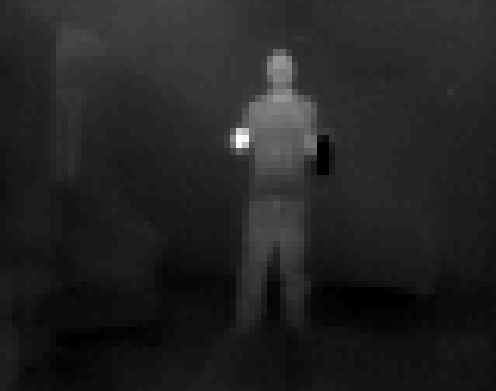
\includegraphics[width=0.5\linewidth]{images/leptonTermalImage.png}
\caption[Obraz człowieka w~termowizji wykonany kamerą Lepton.]{Obraz człowieka w termowizji wykonany kamerą Lepton. W~prawej ręce widać gorący obiekt (kubek herbaty), w~lewej zimny (butelka wody z lodówki).}
\label{fig:leptonTermalImage}
\end{figure}
%OK TODO 2 , ale tradycyjnie - powołanie w tekśie na obraz.



\section{Rejestracja obrazu multispektralnego}

Widmo elektromagnetyczne docierające do kamery składa się fal o~różnych długościach. 
Sensory w~kamerach rejestrują obraz tylko w~pewnym zakresie tego widma, więc aby uzyskać obraz w~wymaganym paśmie należy odfiltrować niepożądane elementy widma, np. kolorowy obraz z kamery wizyjnej jest otrzymywany poprzez zastosowanie trzech filtrów: czerwonego, zielonego i niebieskiego. 
Ponieważ wszystkie trzy kolory mogą być zarejestrowane przez pojedynczą matrycę, filtry są nałożone bezpośrednio na sensor, a~wartość koloru w danym punkcie jest interpolowana z~sąsiadujących ze sobą pikseli (tzw. matryca Bayera). 
W~przypadku, gdy nie jest możliwe zastosowanie jednego sensora do wszystkich pożądanych zakresów, należy rozdzielić wiązkę pomiędzy kilka różnych matryc aparaty, albo wykorzystać równoległy układ kamer. %OK TODO 2 aparaty źle brzmi. Druga sprawa to są takie kamery 3x CMOS, gdzie wiązka jest rozdzialana na trzy czujniki (nie ma tej interpolacji)

W przypadku jednoczesnej rejestracji obrazu wizyjnego i~termicznego większość rozwiązań wykorzystuje układ dwóch równoległych do siebie kamer -- przykład przedstawia rysunek \ref{dual_camera}. 
W tym przypadku została zastosowana kamera termowizyjna FLIR Tao 2 oraz kamera wizyjna Logitech Webcam c600. 

Zazwyczaj obrazy z kamer różnią się, co wynika z ich budowy, różnej rozdzielczości, kąta widzenia oraz zniekształceń soczewkowych.
Do poprawnego odwzorowania tej samej sceny w~obu widmach należy zastosować algorytm mający na celu dopasowanie obu obrazów.
Tworzony jest w~ten sposób nowy obraz, na którym wszystkie piksele łączą informacje o~kolorze i temperaturze.

Pierwszym z~etapów poprawnego dopasowania obrazów jest kalibracja systemu wizyjnego.
Wykonuje się ją z~wykorzystaniem specjalnych plansz, które pozwalają określić położenie pewnych punktów w~przestrzeni w~obu rejestrowanych zakresach promieniowania.
Punkty te pozwalają na obliczenie relacji między obrazami.
Plansze mogą być aktywne (posiadają własne źródło ciepła) albo pasywne (przesłaniają obce źródło ciepła).
W~równoległym układzie kamer występuje również zjawisko paralaksy, które powiększa się wraz ze wzrostem odległości obiektu od punktu kalibracji. Ogranicza to zakres w jakim może działać taki system. %OK TODO 2 to zdanie jest takie na doczepkę. Może napisać co z tego wynika

W~pracy \cite{hwang2015multispectral} autorzy zastosowali zwierciadło półprzezroczyste wykonane z~wafla krzemowego pokrytego cynkiem do rozdzielenia obrazu wizyjnego od termicznego (rysunek \ref{multispectral}). 
Wykorzystując trójosiowy uchwyt, kamery zostały ustawione tak, by ich osie optyczne się pokrywały. 
Następnie obrazy z~obu kamer zostały zrektyfikowane, aby miały tą samą wirtualną ogniskową.

\begin{figure}[h]
\centering
\begin{subfigure}{0.45\textwidth}
\centering
\includegraphics[width=1\textwidth]{images/dual-camera}
\subcaption{\label{dual_camera}}
\end{subfigure}
\begin{subfigure}{0.45\textwidth}
\centering
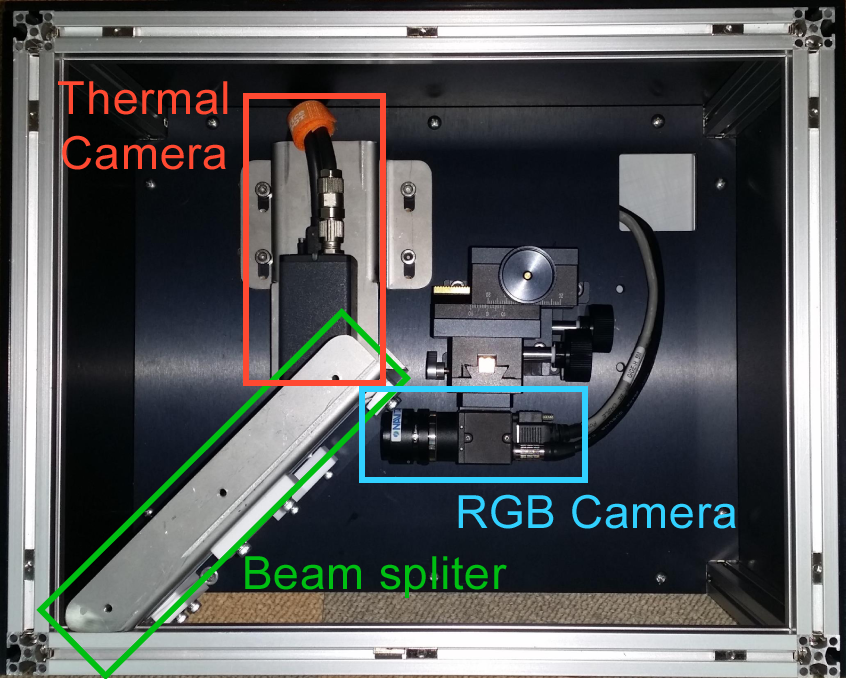
\includegraphics[width=1\textwidth]{images/multispectral}
\subcaption{\label{multispectral}}
\end{subfigure}
\caption{\label{fig:cameras_systems}Sposoby akwizycji obrazów: \protect\subref{dual_camera} dwie kamery równolegle \cite{lee2015robust}, \protect\subref{multispectral} z wykorzystaniem zwierciadła półprzezroczystego \cite{hwang2015multispectral}.}
\end{figure}


\subsection{Model geometryczny}

Do opisu matematycznego systemu wykorzystuje się model kamery otworkowej.
Dzięki niemu można opisać relację między trójwymiarową przestrzenią a~dwuwymiarowym obrazem za pomocą projekcji perspektywicznej. Nie stanowi on najdokładniejszego opisu matematycznego kamery, nie ma w nim uwzględnionych zakłóceń soczewkowych, jednakże zapewnia dobre rezultaty w~większości aplikacji.
Model składa się z~2 zestawów parametrów: zewnętrznych oraz wewnętrznych.
Parametry zewnętrzne definiują lokację kamery względem zewnętrznego układu współrzędnych.
Są reprezentowane przez wektor translacji \(T\) między układem związanym z~kamerą \( \left ( X_{c},Y_{c},Z_{c}\right ) \)
a~zewnętrznym \(\left ( X,Y,Z\right )\).
Drugim parametrem jest macierz rotacji \( R \) (między osiami tych dwóch układów).
Punkt \(P = \left [ X,Y,Z \right ]^T \) będący w~zewnętrznym układzie współrzędnym ma swój odpowiednik w~układzie wewnętrznym, który można określić zależnością:

\begin{equation}
P_{c} = RP+T
\end{equation}

Właściwości optyczne kamery można przedstawić w~postaci macierzy kamery:
\begin{equation}
K = \begin{bmatrix}
f_x & 0 & x_0 \\ 
0 & f_y & y_0\\ 
0 &0 & 1
\end{bmatrix}
\end{equation}
gdzie:
\begin{conditions}
f_{x}, f_{y} & ogniskowa kamery wyrażona w liczbie pikseli, \\
x_{0},y_{0} & współrzędne punktu głównego. 
\end{conditions}

Macierz $K$ określa związek między znormalizowanymi współrzędnymi w~układzie odniesienia kamery danych wzorem \(x_n = \frac{X_c}{Z_c}, y_n = \frac{Y_c}{Z_c}\)  a~odpowiadającym im współrzędnymi punktów na obrazie \(u,v\):

\begin{equation}
\begin{bmatrix}
u \\
v \\
1
\end{bmatrix} = K \begin{bmatrix}
x_n \\
y_n \\
1
\end{bmatrix}
\end{equation}

\subsection{Kalibracja}

Obrazy, które przedstawiają tę samą scenę, ale zostały wykonane dwoma różnymi kamerami w~innych położeniach różnią się. 
Na rysunku \ref{fig:oneSceaneTwoCameras} czarna szachownica jest uchwycona przez dwie kamery ustawione w~punktach $C_A$ (na wprost obiektu) oraz $C_B$ (po skosie i~lekko obrócona).

\begin{figure}
\centering
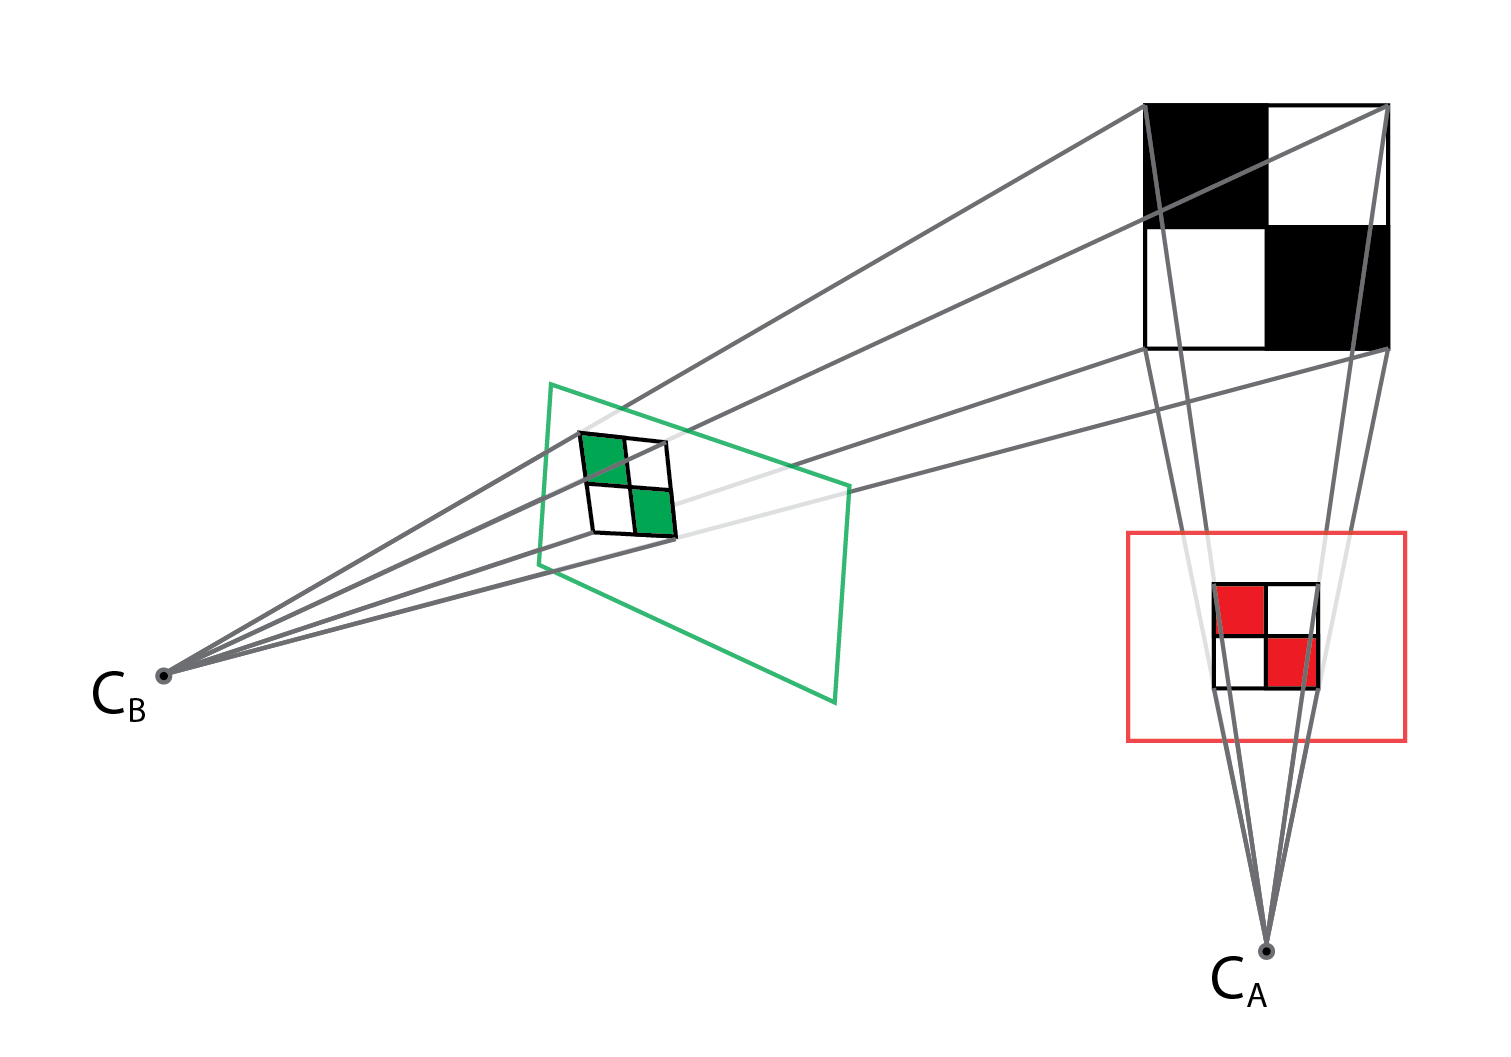
\includegraphics[width=0.6\linewidth]{images/oneSceaneTwoCameras}
\caption[Dwie kamery rejestrujące jeden obiekt. ]{Dwie kamery rejestrujące jeden obiekt.}
\label{fig:oneSceaneTwoCameras}
\end{figure}

Aby dopasować te dwa obrazy, tak by szachownice były ujęte tak samo (tj. w~tym samym miejscu na obrazie), należy na jednym z~nich przeprowadzić transformację projekcyjną. 
Jest to przekształcenie pomiędzy dwoma płaszczyznami, które wykorzystuje model geometryczny kamery. 
Wymaga to uprzedniego wyznaczenia macierzy transformacji $A$ na podstawie co najmniej 4 punktów kalibracyjnych.

\begin{figure}[h]
\centering
\begin{subfigure}{0.30\textwidth}
\centering
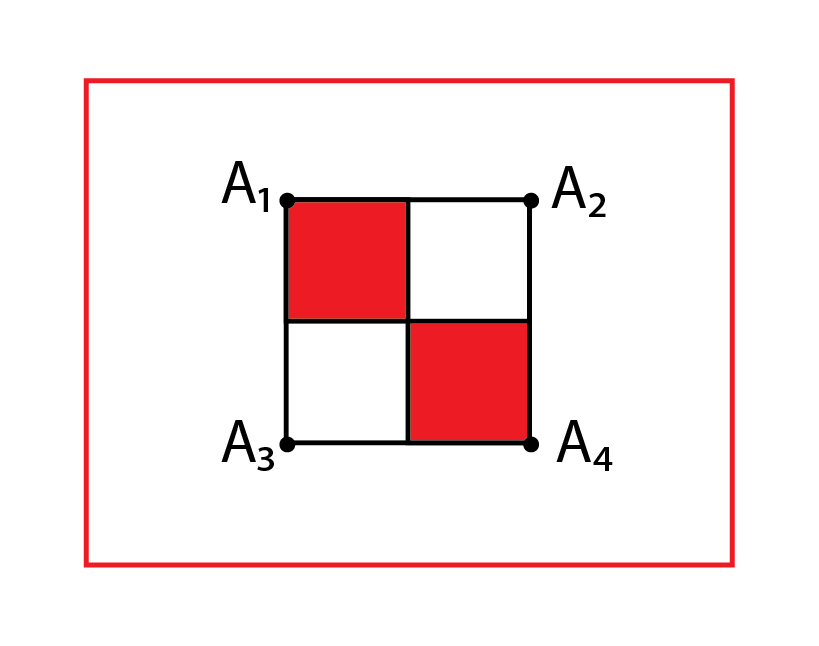
\includegraphics[width=1\textwidth]{images/camAimage}
\subcaption{\label{fig:camAimage}}
\end{subfigure}
\begin{subfigure}{0.30\textwidth}
\centering
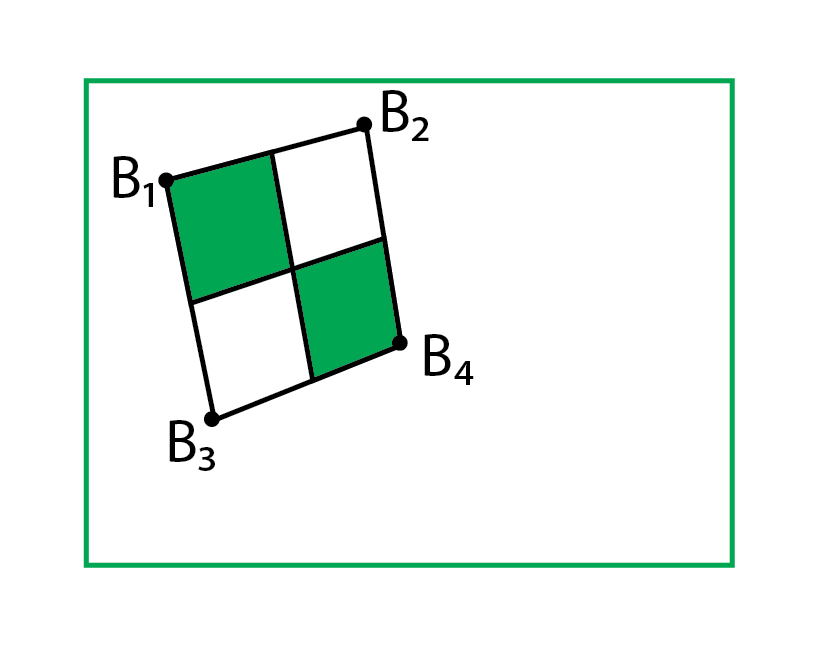
\includegraphics[width=1\textwidth]{images/camBimage}
\subcaption{\label{fig:camBimage}}
\end{subfigure}
\caption{\label{fig:camImages}Zarejestrowane obrazy: \protect\subref{fig:camAimage} przez kamerę $C_A$, \protect\subref{fig:camBimage} przez kamerę $C_B$. Punkty $A$ i $B$ są punktami kalibracyjnymi.}
\end{figure}

Na rysunkach \ref{fig:camAimage} i~\ref{fig:camBimage} punkty $A_1$ do $A_4$, będące czterema rogami zarejestrowanej szachownicy przez kamerę $C_A$, odpowiadają punktom $B_1$ do $B_4$, będącymi tymi samymi czterema rogami zarejestrowanymi kamerą $C_B$. Macierz transformacji $A$ można obliczyć rozwiązując równanie \eqref{transformMatrix}:
\begin{equation}
\label{transformMatrix}
A = \begin{bmatrix}
a & b & c\\ 
d & e & f\\ 
g & h & 1
\end{bmatrix}
\end{equation}

\begin{equation}
\begin{bmatrix}
u_1\\ 
u_2\\ 
u_3\\ 
u_4\\
...\\ 
u_n\\ 
v_1\\ 
v_2\\ 
v_3\\ 
v_4\\ 
...\\ 
v_n 

\end{bmatrix}
=
\begin{bmatrix}
x_1 & y_1 & 1 & 0 & 0 & 0 & -u_1x_1 & -u_1y_1\\ 
x_2 & y_2 & 1 & 0 & 0 & 0 & -u_2x_2 & -u_2y_2\\ 
x_3 & y_3 & 1 & 0 & 0 & 0 & -u_3x_3 & -u_3y_3\\ 
x_4 & y_4 & 1 & 0 & 0 & 0 & -u_4x_4 & -u_4y_4\\ 
...\\ 
x_n & x_n & 1 & 0 & 0 & 0 & -u_nx_n & -u_ny_n\\ 
0 & 0 & 0 & x_1 & y_1 & 1 & -v_1x_1 & -v_1y_1\\ 
0 & 0 & 0 & x_2 & y_2 & 1 & -v_2x_2 & -v_2y_2\\  
0 & 0 & 0 & x_3 & y_3 & 1 & -v_3x_3 & -v_3y_3\\ 
0 & 0 & 0 & x_4 & y_4 & 1 & -v_4x_4 & -v_4y_4\\ 
...\\ 
0 & 0 & 0 & x_n & y_n & 1 & -v_nx_n & -v_ny_n
\end{bmatrix}
\begin{bmatrix}
a \\
b\\
c\\
d \\
e\\
f\\
g\\
h
\end{bmatrix}
\end{equation}

\begin{conditions}
u_{n},v_{n} & współrzędne punktu kalibracji $n$, na obrazie bazowym\\
x_{n},y_{n} & współrzędne punktu kalibracji $n$, na obrazie dopasowywanym 
\end{conditions}

Transformację projekcyjną można zinterpretować jako rzutowanie płaszczyzny, co obrazuję rysunek \ref{fig:projection}. 
Wynikiem transformacji (a~zarazem rzutowania) jest obraz dopasowany do obrazu bazowego (\ref{fig:projectionImage})


\begin{figure}
\centering
\begin{subfigure}{0.47\textwidth}
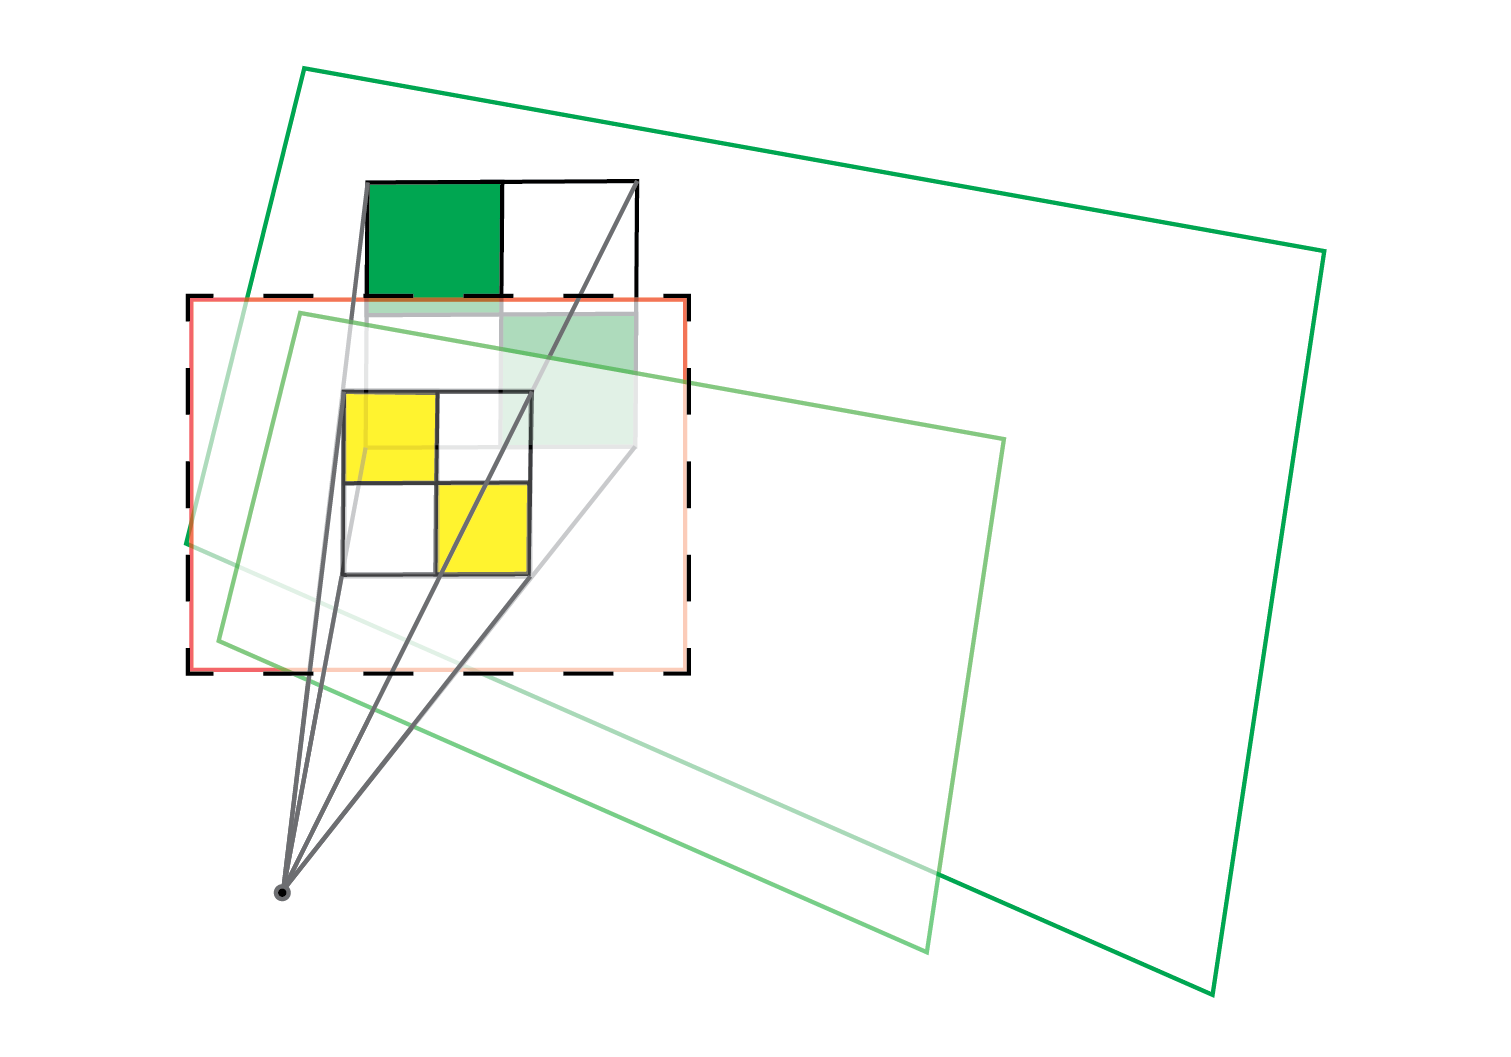
\includegraphics[width=0.9\linewidth]{images/projection}
\caption[Interpretacja transformacji projekcyjnej: rzutowanie płaszczyzny. ]{Interpretacja transformacji projekcyjnej: rzutowanie płaszczyzny.}
\label{fig:projection}
\end{subfigure}
\begin{subfigure}{0.47\textwidth}
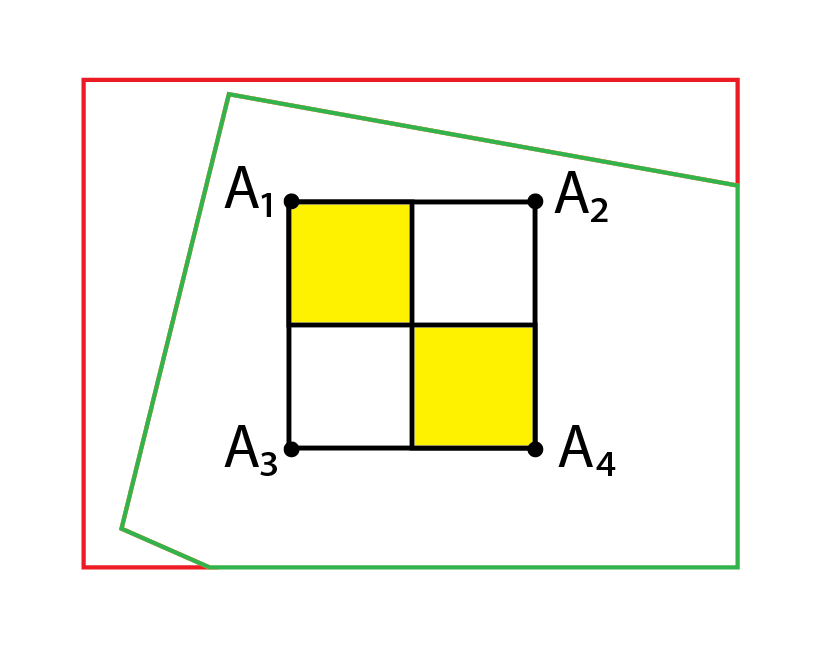
\includegraphics[width=0.9\linewidth]{images/projectionImage}
\caption[Wynik transformacji. ]{Wynik transformacji.}
\label{fig:projectionImage}
\end{subfigure}
\caption[Transformacja projekcyjna ]{Transformacja projekcyjna.}
\end{figure}

\chapter{Algorytmy detekcji pieszych}
\label{cha:algoDetPiesz}

W~cyfrowej analizie obrazu detekcja pieszych jest jedną z~najbardziej aktywnie rozwijanych dziedzin.
W~ciągu kilkudziesięciu lat powstało ponad tysiąc artykułów poruszających to zagadnienie \cite{zhang2015filtered}, w~których zaproponowano wiele różnych metod.
Większość z~nich opiera się na analizie obrazu tylko w~jednym spektrum: widzialnym albo podczerwieni.
Praca \cite{hwang2015multispectral} pokazała, iż połączenie obu obrazów może dać lepsze wyniki.
Podobnie w~artykule \cite{gonzalez2016pedestrian} wykazano, że analiza multispektralna jest skuteczniejsza w~dzień niż w~nocy (o~około 5\% AMR (ang. \textit{Avrange Miss Rate}).
W~artykule \cite{benenson2014ten} autorzy podsumowują osiągnięcia w~dziedzinie detekcji pieszych w latach 2004 -- 2014.
Wyróżniono ponad 40 różnych podejść do problemu.
Eksperymenty w~artykule są oparte o~bazę danych Caltech-USA, która zawiera obrazy w~kolorze.
Jednym z wniosków jest to, że przez ostanie dziesięć lat największy postęp został osiągnięty głównie dzięki dopracowaniu cech, które są wyodrębniane z obrazu, niż ulepszanie klasyfikatora.
Dodatkowo autorzy połączyli cechy dające najlepsze wyniki i~stworzyli własną metodę, która pozwoliła poprawić o~ok 12\% AMR względem najlepszej badanej wcześniej metody.

Coraz większą popularnością cieszą się rozwiązania oparte o głębokie sieci neuronowe  (DNN ang. \textit{Deep Neural Networks}). W artykule \cite{du2017fused} został zaprezentowany system wykrywania pieszych operaty na fuzji kilkunastu dobrze wyuczonych sieci neuronowych, dając jeden z lepszych wyników detekcji z wykorzystaniem bazy Caltech-USA. 
%ok TODO a coś o głębokich sieciach ? Jakoś pominął Pan ten temat.
%ok TODO 2 jw. ? chociaż jeden przykład - bo to jest teraz na topie....

Dla typowego algorytmu detekcji pieszych można wyróżnić trzy podstawowe etapy:

\section{Ustalenie regionu zainteresowania}

Jest to obszar zwany ROI (ang. \textit{Region Of Interest}), w~którym potencjalnie mogą znajdować się piesi.
Wiele podejść uznaje cały obraz jako ROI i~stosuje okno przesuwne, sprawdzając każdy możliwy fragment obrazu.
Jeżeli scena jest rejestrowana przez nieruchomą kamerę, ROI można określić poprzez różnicę między zapamiętanym tłem a~aktualnym obrazem (tzn. modelowanie i~odejmowanie tła). 
Analiza przepływu optycznego również pozwala na wyodrębnienie obszaru, w~których obserwowany jest ruch inny niż na pozostałej części sceny. 
Inną metodą jest zastosowanie słabszego, bardziej ogólnego, ale mniej wymagającego obliczeniowo  klasyfikatora.
Wyodrębnienie ROI jest bardzo istotne w~przypadku pracy w~czasie rzeczywistym, ze względu na ograniczony maksymalny czas analizy pojedynczego obrazu.

\section{Wyodrębnienie cech}

Do najbardziej popularnych cech można zaliczyć:

\begin{enumerate}
\item Histogramy zorientowanych gradientów (HOG ang. \textit{Histogram of Oriented Gradients }).
Algorytm został zaproponowany przez N.Dalala i B. Triggsa w~pracy \cite{dalal2005histograms} i~stał się jedną z~najbardziej popularnych metod w~dziedzinie detekcji ludzi. 
Jest cały czas rozwijany i~modyfikowany w~wielu pracach naukowych.
W pierwszej kolejności zostają obliczone gradienty dla obrazu, za pomocą dwóch masek kierunkowych [-1 0 1] i [-1 0 1]$^T$. Gradienty mogą być ze znakiem lub bez. Na rysunku \ref{fig:hog} przedstawiono przykład uzyskiwania gradientów. Następnie tworzone są histogramy orientacji na podstawie gradientów uzyskanych z pkt. 1. Histogram ma z~góry zadaną liczbę przedziałów i zawiera dane z komórki (ang. \textit{cell}) o określonej wielkości (np. kwadrat 6x6). Wagi orientacji poszczególnych pikseli wynikają z wartości wypadkowej gradientu. Na rysunku \ref{fig:hog2} zaprezentowano przykładowe histogramy.
Komórki łączone są w bloki, w obrębie których następuje normalizacja. Ma ona na celu wyrównanie kontrastów pomiędzy sąsiadującymi blokami komórek. Bloki mają z góry ustalony rozmiar i nakładają się na siebie. Połączenie wszystkich histogramów we wszystkich blokach w jeden wektor cech.

\begin{figure}
\centering
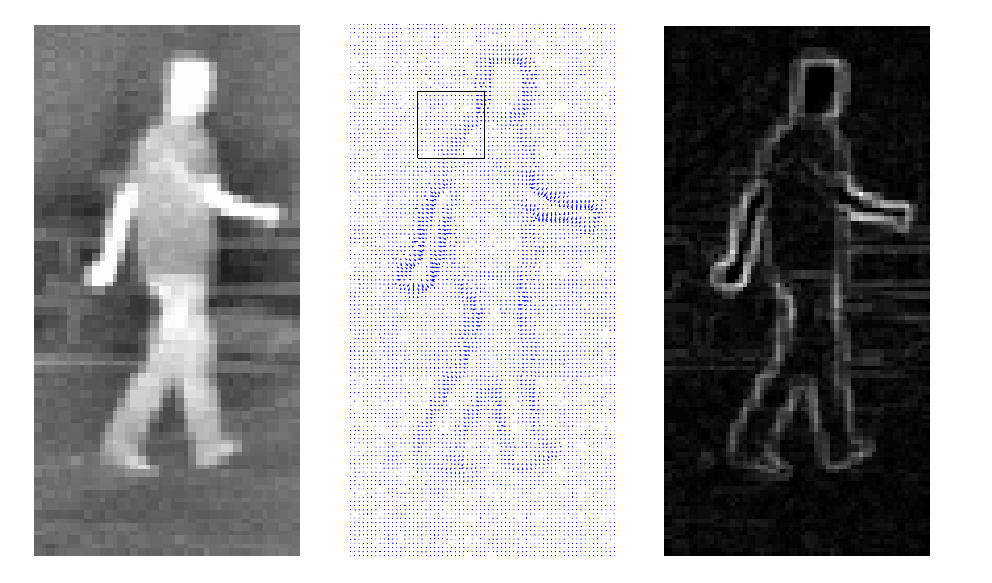
\includegraphics[width=0.5\linewidth]{images/hog}
\caption[Obliczanie gradientów dla obrazu.]{Obliczanie gradientów dla obrazu. Po lewej oryginalny obraz, pośrodku kierunki gradientów, po prawej wartości modułów \cite{suard2006pedestrian}.}
\label{fig:hog}
\end{figure}

\begin{figure}
\centering
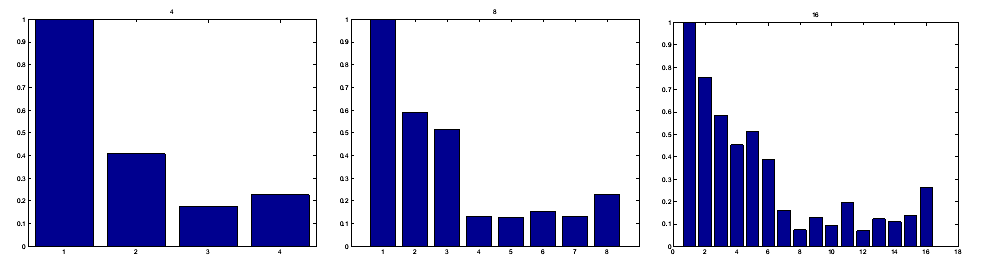
\includegraphics[width=0.7\linewidth]{images/hog2}
\caption[Przykładowe histogramy]{Przykłady histogramów o różnej ilości przedziałów \cite{suard2006pedestrian}.}
\label{fig:hog2}
\end{figure}

%TT w dalszym rozdziale jest to szczegółowo opsane.
%TODO 2 Skoro tak to proszę dać więcej szczegółów 

\item Lokalne wzorce binarne LBP (ang. \textit{Local Binary Paterns}).
Oryginalnie deskryptory te zostały zaproponowane  do opisu tekstur \cite{ojala2002multiresolution}. %OK TODO \cite też coś ojala - 2 tego Pan nie zrobił.
Analizowany obraz zostaje podzielony na bloki.
Następnie, do każdego piksela w~bloku zostaje przypisany wzorzec binarny na podstawie wartości pikseli w~jego sąsiedztwie.
Jeżeli wartość sąsiadującego piksela jest większa od centralnego, to przyjmuje on wartość~1. 
W~ten sposób do każdego piksela przypisywany jest wzorzec binarny (np. 1100110). %OK TODO 2 7 bitów.. raczej 8
Następnie zostaje obliczony histogram wzorców dla każdego bloku.
Histogramy z wszystkich bloków wchodzących w~skład obrazu (okna detekcji) tworzą wektor cech.

\item Falki Haara.
Określają różnicę w~kontraście między dwoma przylegającymi prostokątnymi obszarami. 
W~oryginalnej pracy P.Viola i M.Jones z~2001 \cite{viola2001rapid} autorzy rozważali 3 rodzaje cech: 
\begin{itemize}
	\item dwa obszary mające ten sam rozmiar i~kształt oraz przylegające do siebie horyzontalnie bądź wertykalnie, gdzie cechę stanowi różnica sumy pikseli zawartych w~każdym z regionów ( Układ A i B na rysunku \ref{fig:haar}), 
	\item obszar składający się z 3 prostokątów przylegających do siebie, gdzie od sumy środkowego elementu jest odejmowana suma dwóch zewnętrznych (układ~C),
	\item układ 4 prostokątów, gdzie suma jest różnicą między obszarami po przekątnej (układ~D). %OK TODO 2 niejasne...
\end{itemize}

\begin{figure}
\centering
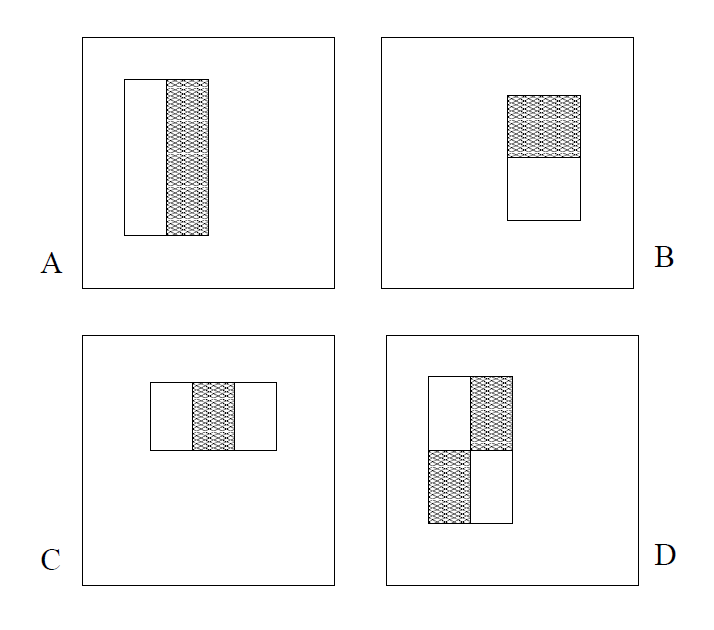
\includegraphics[width=0.4\linewidth]{images/haar}
\caption[Falki Harrra.]{Przykładowe prostokąty służące do określenia cech. Od sumy pikseli zawartych w~białym prostokącie zostaje odjęta suma pikseli w~szarym. \cite{viola2001rapid}.}
\label{fig:haar}
\end{figure}
%OK TODO 2 obrazek by bardzo pomógł
Cechy są łatwe do skalowania i~nie wymagają dużych nakładów obliczeniowych. W celu szybkiego obliczania tych cech stosuje się tzw. \textit{intergral image}. Dla każdego puntu o~współrzędnych x,y zostaje obliczona suma wartości pikseli znajdujących się na lewo i~nad pozycją~x,y. Dzięki temu, aby obliczyć sumę pikseli w~danym kwadracie wystarczą jedynie cztery punkty referencyjne. Na przykład, by obliczyć sumę pikseli w~prostokącie D na rysunku \ref{fig:integralImage} wystarczy rozwiązać równanie $D = 4 + 1 -(2 + 3)$.

\begin{figure}
\centering
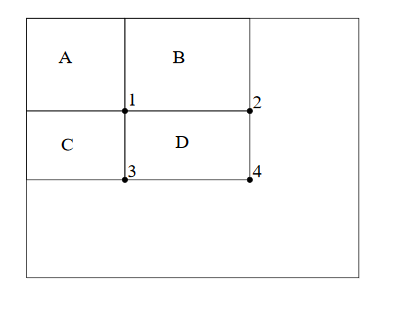
\includegraphics[width=0.4\linewidth]{images/integralImage}
\caption[IntegralImage.]{Obliczanie sumy pikseli za pomocą \textit{integral image}.  \cite{viola2001rapid}.}
\label{fig:integralImage}
\end{figure}
%OK TODO 2 można Pan dodać, że ich do ich obliczania można wykorzystać tzw. intergral image.

\item Kolor. 
W~analizie obrazów wykorzystuje różne przestrzenie barw np. RGB, HSV oraz LUV. 
Głównie wtedy, gdy kolor wykrywanego obiektu jest kluczowy (np. znaki drogowe, światła na skrzyżowaniu). 
Jako cechę można go wykorzystać w~kilku formach. 
Momenty koloru (ang. \textit{Color Moments}) jest to średnia, wariancja i~odchylenie standardowe występowania danego koloru na obrazie. 
Histogram określa częstość występowania danego koloru, a~wektor koherencji koloru (CCV ang. \textit{Color Coherence Vectors}) określa w~jakim stopniu piksele danego koloru są częścią obszaru o~podobnym kolorze (np. obraz zielonej łąki na którym pasie się jedna fioletowa krowa. Kolor zielony na obrazie byłby rozłożony równomiernie natomiast fioletowy byłby skupiony w~pojedynczym rejonie koherencji -- krowy) \cite{kodituwakku2004comparison}.

\end{enumerate}

\section{Klasyfikator}

Otrzymany wektor cech jest następnie poddany klasyfikacji, której wynik decyduje czy obraz zawiera człowieka.
W pracy \cite{benenson2014ten} autorzy wyróżnili 3 dominujące rodziny metod:

\begin{enumerate}
\item Rodzina DPM (ang. \textit{Deformable Part Model})
%
Technika zakłada, że obiekty mogą być zamodelowane poprzez części ułożone w~deformowanych konfiguracjach. 
Model składa się z~głównego, globalnego filtra, który stanowi punkt odniesienia dla pozostałych części. 
Każda część zawiera swój własny filtr wraz z~zestawem dozwolonych pozycji względem okna detekcyjnego oraz koszt deformacji dla każdej z tych pozycji. 
Suma wyniku uzyskanego z~filtra głównego wraz z~jego częściami stanowi o~wyniku detekcji \cite{felzenszwalb2008discriminatively}.

\item Deep networks.
%OK TODO 2 1. Musi Pan wraznie zaznaczyć, że to jest nieco odrebne, w sensie ze to jest ekstrakca + klasyfikacja.
%OK TODO 2 2. Jakiś rysunek by też pomógł.

\begin{figure}
\centering
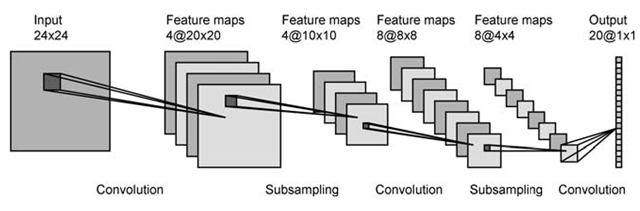
\includegraphics[width=0.8\linewidth]{images/DNN}
\caption[IntegralImage.]{Schemat przykładowej sieci konwolucyjnej.}
\label{fig:DNN}
\end{figure}

Głębokie sieci neuronowe posiadają kilkanaście warstw ukrytych między warstwą wejściową i wyjściową. 
Ich działanie polega na tym, że po podaniu wektora cech na warstwę wejściową wytrenowanej sieci, w~warstwie wyjściowej aktywuje się neutron odpowiedzialny za detekcję danej klasy. 
W~analizie obrazu szczególnie chętnie wykorzystywane są sieci konwolucyjne. W odróżnieniu od klasycznego podejścia głębokie sieci konwolucyjne łączą w sobie oba zadania: wyodrębnianie cech i klasyfikacje.
Neurony pierwszej warstwy ukrytej są podłączone jedynie do wybranego fragmentu warstwy wejściowej (np. okna 24x24). %OK TODO 2 ten histogram jest dla mnie niejasny %To usunę 
Jest to tzw. warstwa konwolucyjna. 
Neurony w~tej warstwie dzielą wspólne wagi dla swoich wejść i bias. 
Sieć posiada zazwyczaj kilkanaście takich warstw -- każda wykrywająca pojedynczą cechę. 
Pozwala to na redukcję liczby neutronów i~parametrów potrzebnych do uzyskania w procesie uczenia. 
Do warstw konwlucyjnych dochodzą warstwy sumujące (ang. \textit{Polling Layers}). 
Ich zadaniem jest generalizacja informacji z poprzedniej warstwy. 
Sieć zamyka warstwa wyjściowa. Na rysunku \ref{fig:DNN} przedstawiono schemat przykładowej sieci konwolucyjnej.
%OK TODO 2 to ostatnie zdanie do uzupełnienia - niejasne.

\item Decision forests

Lasy decyzyjne to zbiory nieskorelowanych drzew decyzyjnych. 
Pojedyncze drzewo jest graficznym odwzorowaniem procesu decyzyjnego. Na podstawie wektora cech drzewo zwraca rozkład prawdopodobieństwa przynależności obiektu do klas. Wynikiem ostatecznym jest średnia prawdopodobieństw z wszystkich drzew w lesie. Rysunek \ref{fig:forest} przedstawia schemat koncepcyjny dla lasu o trzech drzewach.
Algorytm uczenia drzew wykorzystuje przykłady (wektor cech) i związane z nimi konsekwencje (klasyfikacja obiektu).

\begin{figure}
\centering
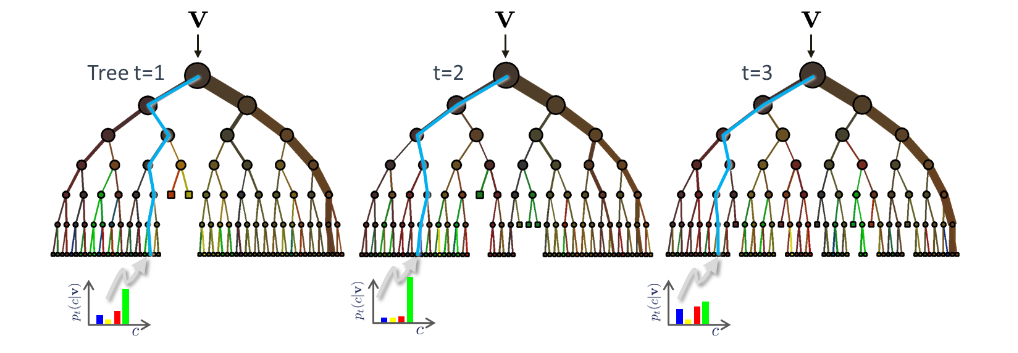
\includegraphics[width=0.9\linewidth]{images/forest}
\caption[Las decyzyjny.]{Schemat lasu decyzyjnego składającego się z trzech drzew \cite{criminisi2011decision}.}
\label{fig:forest}
\end{figure}
%TODO 2 też może rysunek

\item inne: np. SVM (ang. Support Vector Machine -- maszyna wektorów nośnych), AdaBoost itp.


\end{enumerate}

\section{Specyfikacja detekcji w podczerwieni}

Człowiek jest istotą żyjącą, co za tym idzie, wytwarza ciepło. Przeważnie ciało człowieka ma wyższą temperaturę niż otoczenie, co jest wyraźnie widoczne na obrazie termowizyjnym. Termowizja najlepiej sprawdza się w nocy, kiedy kontrast między człowiekiem a otoczeniem jest największy. Ta cecha powoduje, że podczerwień jest chętnie wykorzystywana do systemów wspomagania kierowcy, aby zwiększyć bezpieczeństwo poruszania się po drodze w nocy.  Sylwetka przechodnia może zostać w bardzo prosto wyodrębniona, wykonując prostą operację binaryzacji. Rysunek \ref{fig:binaryzacja} przedstawia przykładowy proces binaryzacji. Daje to możliwość zastosowania wielu algorytmów, które opierają się na kształcie obiektu (np. wzorzec probabilistyczny albo obliczenie proporcji wysokości do szerokości).

\begin{figure}[h]
	\centering
	\begin{subfigure}{0.47\textwidth}
		\centering
		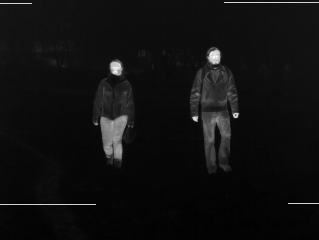
\includegraphics[width=0.9\linewidth]{images/Example_Oryginal}
		\subcaption{\label{fig:Example_Oryginal}}
	\end{subfigure}
	\begin{subfigure}{0.47\textwidth}
		\centering
		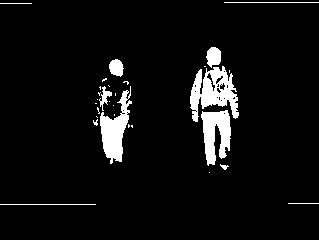
\includegraphics[width=0.9\linewidth]{images/Example_BW}
		\subcaption{\label{fig:Example_BW}}
	\end{subfigure}
	\caption[Przykład binaryzacji]{Binaryzacja: \protect\subref{fig:Example_Oryginal} Obraz zarejestrowany kamerą termowizyjną, \protect\subref{fig:Example_BW} Obraz po binaryzacji\cite{kankaing}.}
	\label{fig:binaryzacja}
\end{figure}

%TODO Nie omówił Pan specyfiki detekcji w podczerwieni.
%TODO 2 Czy specyfika detekcji w podczerwieni gdzies jest ?



\chapter{Wykorzystane zasoby sprzętowe i technologie}
\label{cha:hw}
\section{Kamera termowizyjna Lepton}

\begin{figure}[h]
    \centering
    \includegraphics[width=0.6\textwidth]{images/Lepton}
    \caption{Widok poglądowy na kamere Flir Lepton.}
    \label{fig:lepton}
\end{figure}
 
Lepton jest zintegrowaną w pojedynczym układzie kamerą składającą się z soczewki, sensora podczerwieni fal długich (ang. LWIR – long wave infrared) oraz elektroniki sterującej i przetwarzającej sygnał. Checuje siębardzo małymi wymiarami co czyni go idealnym do zastosowań mobilnych. Układ ma możliwość domontowania dodatkowej przesłony która jest wykorzystywana do automatycznej optymalizacji procesu ujednolicania obrazu (kalibracji sensora).
Prosty do integracji z dowolnym mikrokontrolerem dzięki zastosowaniu standardowych protokołów i interfejsów. Lepton po podłączeniu od razu pracuję w domyślnym trybie pracy, który może zostać zmieniony za pomocą CCI (ang. camera control interface – interfejs kontroli kamery).\cite{lepton}
Parametry:
\begin{itemize}
\item Wymiary: 11,8 x 12,7 x 7,2 mm, 
\item Sensor: niechłodzony mikrobolometr VOx (tlenek wanadu),
\item Rejestrowany zakres: fale długie podczerwieni, 8$\mu m$ do 14$\mu m$ ,
\item Wielkość piksela: 17 $\mu$m,
\item Rozdzielczosć: 80x60 pikseli,
\item Ilość klatek na sekundę 8,6,
\item Zakres rejestrowanych temperatur: -10  $^\circ$  C 140  $^\circ$  C (Tryb wysokiego wzmocnienie),
\item korekta niejednorodności matrycy: automatyczna na bazie przepływu optycznego
\item kąt widzenia horyzontalny / diagonalny: 51 $^\circ$ \\ 66 $^\circ$,
\item Głębia ostrości: od 10cm do nieskończoności
\item Format wyjściowy: do wyboru: 14-bit, 8-bit (z AGC (ang. automatic gain control – automatyczna kontrola wzocnienia)) 24-bit rgb (z ACG i koloryzacją).
\item Interfejs video: VoSPI (Video over Serial Peripherial Interface)
\item Interfejs sterujący: CCI (I2C podobny)
\end{itemize}
\section{Zynq-7000}

Rodzina układów Zynq-7000 bazuje na architekturze SoC (ang. System on Chip). Posiadają zintegrowany kompletny system składający podzielonego na dwie części: systemu procesorowego bazującego na procesorze ARM Cortex-A9 (PS ang. Porcessing System) oraz logikę programowalną (PL ang. programable logic) FPGA w jednym układzie scalonym. Na rysunku \ref{fig:zynq7000} przedstawiono schemat architektury. Prócz procesora cześć procesorowa posiada wbudowaną pamięć, kontroler pamięci zewnętrzne oraz szereg interfejsów dla układów peryferyjnych takich jak USB, GigEthernet, CAN, I2C, SPI. W części logiki programowalnej znajdują się bloki logiki konfigurowalnej (CLB ang. configurable logic block), 36Kb bloki pamięci RAM, procesory sygnałowe DSP48, układ JTAG, układy zarządzania zegarami oraz dwa 12-bitowe przetwornik analogowo-cyfrowy.

Komunikacji między częścią procesorową a logiką programowalną odbywa się za pośrednictwem Interfejsu AXI (ang. Advanced Extensible Interface), oraz bezpośrednio wykorzystując porty generalnego przeznaczenia, przerwania, oraz poprzez bezpośredni dostęp do pamięci (DMA ang. Direct Memory Access) 

\begin{figure}[h]
    \centering
    \includegraphics[width=1\textwidth]{images/Zynq-7000-Overview}
    \caption{Schemat ogólny architektury układu Zynq-7000.}
    \label{fig:zynq7000}
\end{figure}

\section{Interfejs AXI}
 AXI (ang. Advanced eXtensible Interface zawansowany rozszerzalny interfejs) jest częścią ARM AMBA (ang. Advanced Microcontroller Bus Architecture) – otwartego standardu, specyfikacją do zarządzania i połączeń między blokami funkcyjnymi w SoC. Aktualnie jest stosowana AMBA 4.0 która wprowadziła drugą wersję AXI, AXI4. Występują trzy typy interfejsów dla AXI4:
\begin{itemize}
\item AXI4 – stosowany w wysokowydajnych transferach w przestrzeni pamięci (ang. memory-mapped)
\item AXI4-Lite – stosowany dla prostszych operacji w przestrzeni pamięci (na przykład do komunikacji z rejestrami kontrolnymi i statusu)
\item AXI4-Stream – stosowany do wysokiej prędkości transmisji strumieniowych
\end{itemize}
Specyfikacja interfejsu zakłada komunikację pomiędzy pojedynczym AXI master i pojedynczym AXI slave, która ma na celu wymianę informacji pomiędzy tymi dwoma blokami funkcyjnymi IP core. Kilkanaście interfejsów AXI master i slave mogą zostać połączone między sobą za pomocą specjalnej struktury zwanej interconnect block (blok międzypołączeniowy) w której odbywa się trasowanie połączeń do poszczególnych bloków. 

AXI4 i AXI4-Lite składają się z 5 różnych kanałów:
\begin{itemize}
\item Kanał adresu odczytu,
\item Kanał adresu zapisu,
\item Kanał danych odczytanych
\item Kanał danych do zapisania
\item Kanał potwierdzenia zapisu
\end{itemize}
Dane mogą płynąć w obie strony pomiędzy master a slave jednocześnie. Ilość danych które można przesłać w jednej transakcji w przypadku AXI4 wynosi 256 transferów, zaś AXI4-Lite pozwala na tylko 1 transmisję.

AXI4-Stream nie posiada pola adresowego, a dane mogą być przesyłane nieprzerwanie. 
\section{Wykorzystanie AXI-Stream do transmisji sygnału video.} 
W odróżnieniu od klasycznej implementacji przetwarzania strumieniowego video, w AXI-Stream przesyłane są jedynie aktywne piksele. Linie synchronizacji poziomej i pionowej są odrzucane albo są połączane do specjalnego bloku detekcji timingów który mierzy parametry wchodzącego strumienia wizyjnego (ilość pikseli na linie, czas ilość aktywnych linii, czas wyciemnienia itd.). Podobnie informacje o synchronizacji są dodawane przez blok generujący timingi.

Do transmisji wykorzystane jest 6 linii: jedna linia danych i pięć kontrolno-sterujących. 
\begin{itemize}
\item Video Data – linia danych o szerokości jednego (albo dwóch) pikseli. Szerokość tej linii powinna być wielokrotnością liczby oseim (16, 24, 48 itd.)
\item Valid – Linia podająca czy dane piksela są poprawne,
\item Ready – Linia kontrolna informująca urządzenie master że slave jest gotowy do transmisji danych,
\item Start Of Frame – linia która wskazuje pierwszy piksel nowej ramki,
\item End Of Line – linia wskazująca ostatni piksel w linii.
\end{itemize}
Aby mógł wystąpić poprawny transfer danych linie Valid i Ready muszą być w stanie wysokim podczas rosnącego zbocza zegara. Przykładowe nawiązanie transmisji przedstawia rysunek \ref{fig:handshake}

\begin{figure}[h]
    \centering
    \includegraphics[width=1\textwidth]{images/axi-stream_hendshake}
    \caption{Przykład rozpoczęcia transmisji Reday/Valid.}
    \label{fig:handshake}
\end{figure}

\section{AXI VDMA}
Wiele aplikacji wizyjnych wymaga przechowania całej ramki obrazu w celu jej dalszej obróbki np. podczas skalowania, przycinania bądź dopasowania ilości klatek na sekundę. Część programowalna układu Zynq zazwyczaj nie posiada wystarczającej liczby zasobów do przechowanie klatki obrazu w swojej strukturze. W tym celu jest wykorzystywany mechanizm bezpośredniego dostępu do pamięci który pozwala na przesłanie i wczytanie danych z logiki programowalnej do pamięci RAM bez konieczności angażowania procesora. Realizuje się to poprzez IP-Core AXI VDMA. Zapewnia on przejście między interfejsem AXI4-Stream a AXI4 Memory Map w obu kierunkach. Przed rozpoczęciem przesyłania IP-Core jest konfigurowany poprzez interfejs AXI4-Lite. Konfiguracja zawiera adres w pamięci RAM do którego ma być zapisana bądź wczytana ramka obrazu. Po wgraniu do pamięci ramki kontroler może wywołać przerwanie dla systemu procesorowego.
\chapter{Realizacja}
\label{cha:real}
W celu rozpoznania przechodnia został użyty połączony obraz termowizyjny (IR) i kolorowy (RGB) nazywany dalej RGBIR. Następnie ten obraz zostaje poddany analizie HOG oraz klasyfikacji za pomocą SVM. W celu ustalenia obszaru zainteresowania na obrazie termowizyjnym za pomocą wzorca probabilistycznego zostają wytypowani kandydaci.

\section{Akwizycja obrazu}
Obraz kolorowy służy jako obraz bazowy. Rozdzielczości 640 x 480 pikseli, prędkością 30 klatek na sekundę i głębi 8 bitów na kanał. Źródłem tego obrazu jest kamera podłączona do układu za pomocą interfejsu HDMI. Na obraz bazowy zostaje nałożony obraz termowizyjny z kamery Lepton, który różni się znacząco parametrami. Abu je zsynchronizować zastosowano bufor ramki, do którego jest zapisywany obraz z prędkością 9 klatek na sekundę a odczytywany z prędkością 30. Kolejnym przekształceniem jest transformacja projekcyjna. Ma na celu powiększenie i dopasowanie obrazu by poprawnie pokrywał się z obraz wizyjnym. W tym celu został zaimplementowany moduł który oblicza na podstawie parametrów macierzy transformaty i koordynatami piksela obrazu źródłowego odpowiadającą mu pozycję na obrazie termowizyjnym zapisanym w buforze ramki. Następny moduł dokonuje interpolacji dwuliniowej. Do poprawnej interpolacji wymagane są 4 piksele otaczające obliczony z projekcji punkt. W celu zredukowania liczby dostępów do pamięci i zwiększenie szybkość działania moduł zapamiętuje 4 ostatnio użyte wartości pikseli. Rozwiązanie to pozwala na pracę w czasie rzeczywistym małym kosztem zasobów układu.
Strumień wizyjny jak i termowizyjny działają w AXI-Stream. Umożliwia to łatwą synchronizację obu obrazów na podstawie sygnału SOF (ang. Start o frame). Moduł synchronizacji czeka na pojawienie się tego sygnału w strumieniu termowizyjnym. Do tego momentu wszystkie napływające piksele są odrzucane. Gdy pojawi się sygnał strumień IR zostaje zatrzymany i czeka na pojawienie się sygnału SOF w bazowym strumieniu wizyjnym. Po jego wykryciu strumień IR rusza. Oba strumienie zostają zsynchronizowane tworząc strumień wizyjna obrazu RGBIR. Następnie ten strumień zostaje przesłany do pamięci za pośrednictwem VDMA oraz (po koloryzacji i nałożeniu) wyświetlony na monitorze przez port VGA.

\section{Kalibracja}
Aby obraz termowizyjny poprawnie pokrywał się z obrazem RGB należy wykonać procedurę kalibracji. Kalibracja przeprowadzana jest ręcznie. Oprogramowanie kamery pozwala na zapisanie na karcie SD specjalnego obrazu kalibracyjnego w którym jest zawarty zrzut aktualnie wyświetlanego obrazu wraz z nieprzetworzonym projekcyjnie obrazem IR. Następnie w pakiecie Matlab zostaje obliczona macierz transformaty projekcyjnej za pomocą wbudowanej funkcji. Wymaga ona wskazania 4 par odpowiadających sobie punktów na obrazie RGB oraz IR. Nową macierz można wgrać podając jej parametry w konsoli. 


\section{Wyznaczanie ROI}
Strumień IR z kamery zostaje zbinearyzowany i zbadany w detektorze DPM kożystającym z wzorca probabilistycznego. Moduł DPM przesyła do pamięci listę koordynatów kandydatów wraz z mocą dopasowania. Moduł DPM został zaczerpnięty z pracy inżynierskiej. Moduł wykorzystuję strumień bezpośrednio z kamery. Wielkość okna detekcji wynosi 16 x 40 pikseli. Jeżeli badany obraz binarny wykazał odpowiedni poziom dopasowania do wzorca zostaje wysłana o tym informacja poprzez AXI-Stream do pamięci. Informacja zawiera koordynaty okna w układzie odniesienia kamery IR oraz wartość mocy dopasowania. Gdy zostanie zbadane ostatnie okno w obrazie zostaje wysłany sygnał TLAST co wygeneruje przerwanie dla systemu procesorowego.

\section{Klasyfikacja za pomcą SVM}
Z lisy kandydatów wygenerowanej przez moduł DPM wybierany jest wynik o najwyższej mocy dopasowania. Koordynaty z układu odniesienia kamery zostają poddane transformacie projekcyjnej do układu odniesienia kamery RGB. Z obszaru na obrazie RGBIR zawierającym potencjalnie człowieka zostają wyodrębnione cechy HOG które następnie służą jako wektor dla SVM.

Klasyfikator został opracowany i nauczony na podstawie 60 wyselekcjonowanych obrazów. 30 z nich stanowiło próbką pozytywną zawierającą osobę a 30 nie. Nauczanie zostało zrealizowane przy użyciu oprogramowania Matlab. Próbki pozytywne zostały wygenerowane poprzez zapis ROI wyznaczonych przez wzorzec probabilistyczny. 

\section{Prezentacja wyników}
Na wyjściu konsoli zostają podane współrzędne oraz moc dopasowania i klasyfikacja obiektu. Na obrazie wyjściowym VGA obszar ten zostaje zaznaczony zieloną ramką. Jeżeli potencjalny obszar nie został zakwalifikowany jako człowiek ale miał największą moc dopasowania DPM to obszar zostaję zaznaczony czerwoną ramką. Czarna ramka oznacza że nie został wykryty żaden obiekt. 

Mając do dyspozycji układ heterogeniczny rodziny Zynq-7000 od firmy Xilinx operacje zostały podzielone między programowalną logiką a systemem procesorowym. Ogólny zarys systemu został przedstawiony na rysunku \ref{fig:systemwizyjny}.

\begin{figure}[h]
    \centering
    \includegraphics[width=1\textwidth]{images/system}
    \caption{Schemat blokowy systemu detekcji.}
    \label{fig:systemwizyjny}
\end{figure}

Programowalna logika:
\begin{itemize}
\item Akwizycja Obrazu poprzez HDMI (RGB) i VoSPI (IR),
\item Transformata projekcyjna i interpolacja obrazu IR,
\item Nałożenie i synchronizacja obrazu IR do obrazu RGB,
\item Prezentacja wyników,
\item Detekcja kandydatów za pomocą wzorca probabilistycznego.
\end{itemize}
System Procesorowy:
\begin{itemize}
\item konfiguracja parametrów systemu wizyjnego w logice programowalnej poprzez interfejs AXI-Lite,
\item Klasyfikacja obszarów wytypowanych przez wzorzec probabilistyczny,
\item Generowanie oznaczników.
\end{itemize}

\section{Opis modułów}
\subsection{Kontroler kamery IR}
Pobiera obraz z kamery poprzez interfejs VoSPI który następnie zostaje zapisany do dwuportowej pamięci BRAM. Kontroler na początku pracy wystawia pin CS (ang. Chip Select) w stan niski a po chwili rozpoczyna transmisję poprzez taktowanie zegarem SCK. Kamera na reaguje na opdające zbocze zegara i wystawia kolejny bit danych na swoim porcie MISO. Strumień VoSPI składa się z 63 pakietów na ramkę obrazu. Pakiet rozpoczyna identyfikator składający się z numeru linii oraz sumy CRC pakietu (2 bajty na numer linii i 2 na sumę). Dane pakietu stanowi 160 bajtów – po dwa bajty na piksel w linii. Dane są przesyłane w 14-bitową wartość piksela oraz 2 zera wypełnienia. W przypadku niepoprawnej ramki numer identyfikator przyjmuje wartość xFxx. Ostatnie trzy pakiety stanowią telemetrie i są ignorowane.

\subsection{Transformata projekcyjna}
Moduł zamienia współrzędne z układu odniesienia kamery RGB odpowiadającym im na obrazie IR. Na wejściu podawany jest strumień AXI4-Stream zawierający timingi oraz 12 bitowe współrzędne X i Y. Moduł realizuję operację: 

\begin{equation}
\begin{bmatrix}
u_n & v_n & n
\end{bmatrix} 
= 
\begin{bmatrix}
x & y & 1
\end{bmatrix}
T
\end{equation}

\begin{equation}
u = \frac{u_n}{n}
\end{equation}

\begin{equation}
v = \frac{v_n}{n}
\end{equation}

Moduł wystawia na wyjściu strumień timingów, 12 bitowe wartości U i V oraz ich części ułamkowe w U\_fraction i V\_fraction (14bitów). W module zostały wykorzystane 34 z 80 dostępnych w układzie Zynq procesorów DSP48 do wykonania operacji arytmetycznych. Najwięcej zasobów jest pochłonięte przez IP core dzielarki dostarczony od producenta układu. Do implementacji jednej dzielarki zostało wykorzystane14 modułów DSP. Dzielenie nie odbywa się w pełni potokowo. Użyty w dzielarce algorytm High\_Radix wymaga zatrzymanie strumienia na czas obliczeń. Jednak dzięki zastosowaniu wyższej częstotliwości niż zegar pikseli obrazu RGB oraz bufora (250 MHz) nie stanowi to wąskiego gardła systemu. Macierz T jest zapisana  w dziewięciu 32 bitowych rejestrach i konfigurowalna poprzez interfejs AXI4-Lite. Elementy macierzy są 25 liczbami w notacji stałoprzecinkowej: 1 bit znaku 10 – część całkowita, 14 – część ułamkowa.



\subsection{Interpolacja bilinearna}
Prosty moduł przeznaczony głównie do powiększania obrazów. PoModuł ma za zadanie pobrać z pamięci dwuportowej obrazu IR wartość piksela wskazaną na wejściu układu i wystawić na wyjście. Podobnie jak reszta systemu używa AXI4-Stream do przekazywania danych między poszczególnymi modułami. Dane na wejściu to współrzędne U i V oraz ich części ułamkowe U\_fraction i V\_fraction. Moduł został wyposażony w 4 rejestry w których przechowywane są współrzędne oraz wartości 4 ostatnio użytych pikseli. Zabieg ten znacznie redukuje ilość potrzebnych zapytań do pamięci. Podczas powiększania obrazów jest duża szansa że kolejne koordynaty na wejściu UV odwołują się do tych samych czterech otaczających ich pikseli. W module jest sprawdzane czy w pamięci już są wartości z koordynatów [U,V], [U+1,V] [U,V+1], [U+1,V+1]. Jeżeli któregoś piksela brakuje jest on pobierany z pamięci i zapisywany w rejestrze przechowującym niepotrzebny piksel. Jeżeli wszystkie koordynaty się zgadzają , obliczana jest wartość piksela wyjściowego z wzoru \ref{equ:bilinear}.  
\begin{equation}\label{equ:bilinear}
Ir = A(1-U_f)(1-V_f)+BU_f(1-V_f)+C(1-U_f)V_f+ D U_fV_f
\end{equation}
\noindent gdzie: $ A, B, C ,D $ odpowiadają wartościom pikseli w [U,V], [U+1,V] [U,V+1], [U+1,V+1] a $ Ir $ to wartość wyjściowa piksela wyjściowego. $U_f$ i $V_f$ stanowią U\_fraction i V\_fraction.

Moduł działa strumieniowo. W przypadku gdy jest wymagana aktualizacja rejestrów strumień jest wstrzymywany.
biera wartość 4 otaczających, podanych na wejściu punktu, pikseli z BRAM i na ich bazie jest wykonywana interpolacja. Moduł zapamiętuje 4 ostatnio użyte piksele które są na bieżąco aktualizowane wraz z zmianą położenia punktu wejściowego na obrazie IR.
\subsection{Łączenie strumieni}
Moduł posiada dwa wejścia dla obrazu. Jeden strumień jest głównym i do niego jest dołączany drugi strumień. Do synchronizacja strumieni została wykorzystana możliwość AXI4-Strem do wstrzymania transmisji. Piksele z dołączanego strumienia są odrzucane do momentu pojawienia się sygnału SOF. W momencie pojawienia się sygnału SOF w strumieniu głównym transmisja zostaje wznowiona, pod kontrolą strumienia wyjściowego. Po przejciu całej ramki strumienie są ponownie synchronizowane.  
\subsection{Koloryzacja i nakładanie}
Strumień RGBIR zostaje połączone w jeden obraz. Obraz IR zostaje poddany koloryzacji na podstawie 12-bitowego LUT i nałożony w proporcjach 50 na 50 z obrazem RGB. Na wyjciu jest podany 24 bitowy strumień RGB.

\subsection{Obramowanie wyników}
Moduł dodaje do obrazu podanego na strumień wejściowy ramkę która następnie jest podawana dalej strumieniem wyjściowym. Parametry ramki są ustawiane przez dwa 32 bitowe rejestry. Pierwszy, -position\_reg-, zawiera pozycję gdzie ma się znajdować ramka na obrazie (lewy górny róg ramki), drugi -parameters\_reg- rejestr odpowiada za kolor i wielkość ramki. Rejestry są konfigurowane poprzez AXI4-Lite.

\section{System procesorowy}

System procesorowy spełnia dwa podstawowe zadania: konfiguracja modułów zawartych w logice programowalnej za pomocą interfejsu AXI4-Lite takich jak macierz projekcji, wartość progu binaryzacji i wartość progu mocy dopasowania dla modułu DPM, wzmocnienie oraz offset modułu normalizacji sygnału IR. Pozwala on również na zapisanie na karcie SD aktualną ramkę bądź pozytywnie sklasyfikowany obraz okna detekcyjnego, jak i obrazu do przeprowadzenia kalibracji.

Drugim podstawowym zadaniem jest przeszukanie listy kandydatów w celu znalezienia tego z największą mocą dopasowania, wyliczenie cech HOG i klasyfikacji SVM. Oryginalny rozmiar okna detekcji w układzie kamery IR wynosi 16x40 zaś na obrazie RGBIR analizowane jest okno 80x192 piksele. Okno jest podzielone na 60 komórek o wielkości 16x16 pikseli. Następnie są obliczane gradienty oraz histogram dla każdej komórki. Wykorzystany jest histogram ważony o 9 przedziałach. Do każdego histogramu jest przypisany dodatkowo suma kwadratów wszystkich wartości przedziałów. Następnie komórki są łączone w bloki 2 na 2 w obrębie którego dokonuje się normalizacji wykorzystując wcześniej obliczone sumy kwadratów. Bloki nakładają się na siebie dając w sumie 44 bloki. Suma histogramów z wszystkich bloków tworzy 1584 elementowy wektor cech. Wektor jest przemnożony przez wektor beta uzyskany w procesie nauczania SVM i dodany bias. Jeżeli uzyskany wynik jest większy od 0 badane okno zostaje sklasyfikowane z wynikiem pozytywnym.


\chapter{Wyniki i wnioski}
%TODO OK to trzeba dołączyć do tego poprzedniego rozdziału.


Aby sprawdzić działanie i dokładność systemu została zaimplementowana możliwość zapisu obliczonego wektora cech na karcie SD. 
Następnie został obliczony przykładowy błąd względny między wektorem cech wyliczonym w implementacji programowej, a uzyskanym z sytemu wizyjnego. %TODO jak programowej, to tu bym się spodziewał czegoś a'la sprzętowej 
Błąd oscyluje w granicy \(10^{-6}\) co czyni go marginalnym i najprawdopodobniej wynika z różnić użytych bibliotek numerycznych.
%TODO To jest niejasne. Rozumiem, że to tylko pokazuje, że ARM i Intel coś inaczej liczną ?

<TU WSTAW WYKRES>

Na przebadanie jednego okna zaproponowany system procesorowy potrzebuje 75ms  (dla porównania te same obliczenia w pakiecie Matlab zajmują około 23 ms).
%TODO podać na jakim sprzęcie 
Dzięki zastosowaniu sprzętowego wyszukiwania ROI zadanie sytemu procesorowego zostało ograniczone do obliczenia jednego okna z największym prawdopodobieństwem zawierania w sobie przechodnia. %TODO styl. to zawierania w sobie, poza tym - dalczego akurat tylko jednego.
Kamera termowizyjna, będąca źródłem sygnału dla wzorca probabilistycznego, pracuje z prędkością 9 klatek na sekundę dając w przybliżeniu 111 ms na zbadanie danego okna więc system procesorowy mieści się w tych ramach czasowych z dużym zapasem. %TODO dając - słabe słowo
%TODO  no ale jakby to dla 30/60 fps... to już tak pięknie nie jest

\begin{table}[]
\centering
\caption{Wykorzystane zasoby logiki programowalnej.}
\label{tab:resources}
\begin{tabular}{|l|l|l|l|}
\hline
Resource & Utilization & Available & Utilization \% \\ \hline %TODO po polsku
LUT & 12583 & 17600 & 71,49 \\ \hline 
LUTRAM & 617 & 6000 & 10,28 \\ \hline 
FF & 19924 & 35200 & 56,60 \\ \hline
BRAM & 25,50 & 60 & 42,50 \\ \hline
DSP & 36 & 80 & 45,00 \\ \hline
IO & 43 & 100 & 43,00 \\ \hline
BUFG & 7 & 32 & 21,88 \\ \hline
MMCM & 1 & 2 & 50,00 \\ \hline
PLL & 1 & 2 & 50,00 \\ \hline
\end{tabular}
\end{table}


%TODO Podsumowanie oraz wskazanie dalszych kierunków pracy
%TODO Dodatek A - spis zawartości CD
%TODO Dodatek B - opis informatyczny projektu


\printbibliography

\end{document}
